% !TeX root = main.tex

\chapter{Discrete Fourier Transform}
\glsresetall
\label{chapter:dft}

%\note{Make sure to use consistent notation. E.g., use bold capital letters for matrices.}

The \gls{dft} plays a fundamental role in digital signal processing systems. It is a method to change a discrete signal in the time domain to the same signal in the frequency domain.  By describing the signal as the sum of sinusoids, we can more easily compute some functions on the signal, e.g., filtering and other linear time invariant functions.  Therefore, it plays an important role in many wireless communications, image processing, and other digital signal processing applications.

This chapter provides an introduction to the \gls{dft} with a focus on its optimization for an FPGA implementation. At its core, the \gls{dft} performs a matrix-vector multiplication where the matrix is a fixed set of coefficients. The initial optimizations in Chapter \ref{subsec:dft_implementation} treat the \gls{dft} operation as a simplified matrix-vector multiplication. Then, Chapter \ref{subsec:dft_implementation} introduces a complete implementation of the \gls{dft} in \VHLS code. Additionally, we describe how to best optimize the \gls{dft} computation to increase the throughput. We focus our optimization efforts on array partitioning optimizations in Chapter \ref{subsec:dft_array_partitioning}.

%The \term{Fast Fourier Transform} (\gls{fft}) is a highly optimized method to calculate the \gls{dft}. We will focus on the \gls{fft} in the next chapter.

There is a lot of math in the first two sections of this chapter. This may seem superfluous, but is necessary to fully comprehend the code restructuring optimizations, particularly for understanding the computational symmetries that are utilized by the \gls{fft} in the next chapter. That being said, if you are more interested in the HLS optimizations, you can skip to Chapter \ref{subsec:dft_implementation}. 

\section{Fourier Series}

In order to explain the discrete Fourier transform, we must first understand the \term{Fourier series}. The Fourier series provides an alternative way to look at a real valued, continuous, periodic signal where the signal runs over one period from $-\pi$ to $\pi$. The seminal result from Jean Baptiste Joseph Fourier states that any continuous, periodic signal over a period of $2 \pi$ can be represented by a sum of cosines and sines with a period of $2 \pi$. Formally, the Fourier Series is given as

\begin{equation}
\begin{array} {lcl} 
f(t) & \sim &  \frac{a_0}{2} + a_1 \cos (t) + a_2 \cos (2t) + a_3 \cos (3t) + \dots \\
& & + b_1 \sin(t) + b_2 \sin(2t) + b_3 \sin(3t) + \dots \\
& \sim & \frac{a_0}{2} + \displaystyle\sum\limits_{n=1}^{\infty} (a_n \cos (nt) + b_n \sin(nt))
\end{array}
\label{eq:fourier_series}
\end{equation}
where the coefficients $a_0, a_1, \dots$ and $b_1, b_2, \dots$ are computed as

\begin{equation}
\begin{array} {lcl} 
a_0 & = & \frac{1}{\pi} \int_{-\pi}^\pi f(t)\,\mathrm{d}t \\
a_n & = & \frac{1}{\pi} \int_{-\pi}^\pi f(t) \cos(nt)\,\mathrm{d}t \\
b_n & = & \frac{1}{\pi} \int_{-\pi}^\pi f(t) \sin(nt)\,\mathrm{d}t \\
\end{array}
\label{eq:fourier_coefficients}
\end{equation}

There are several things to note. First, the coefficients $a_0, a_1, a_2, \dots, b_1, b_2, \dots$ in Equation \ref{eq:fourier_coefficients} are called the Fourier coefficients. The coefficient $a_0$ is often called the \term{direct current (DC)} term (a reference to early electrical current analysis), the $n=1$ frequency is called the fundamental, while the other frequencies ($n \ge 2$) are called higher harmonics. The notions of fundamental and harmonic frequencies originate from acoustics and music. Second, the function $f$, and the $\cos()$ and $\sin()$ functions all have a period of $2 \pi$; changing this period to some other value is straightforward as we will show shortly. The DC value $a_0$ is equivalent to the coefficient of $\cos (0 \cdot t) = 1$, hence the use of symbol $a$. The $b_0$ value is not needed since $\sin (0 \cdot t) = 0$. Finally, the relation between the function $f$ and its Fourier series is approximate in some cases when there are discontinuities in $f$ (known as Gibbs phenomenon). This is a minor issue, and only relevant for the Fourier series, and not other Fourier Transforms. Therefore, going forward we will disregard this ``approximation'' ($\sim$) for ``equality'' ($=$). 

Representing functions that are periodic on something other than $\pi$ requires a simple change in variables. Assume a function is periodic on $[-L, L]$ rather than $[-\pi, \pi]$. Let 
\begin{equation}
t \equiv \frac{\pi t'}{L}
\end{equation} and 
\begin{equation}
\mathrm{d}t = \frac{\pi \mathrm{d}t'}{L}
\end{equation} which is a simple linear translation from the old $[-\pi, \pi]$ interval to the desired $[-L, L]$ interval.
Solving for $t'$ and substituting $t' = \frac{L t}{\pi}$ into Equation \ref{eq:fourier_series} gives
\begin{equation}
f(t') = \frac{a_0}{2} + \displaystyle\sum\limits_{n=1}^{\infty} (a_n \cos (\frac{n \pi t'}{L}) + b_n \sin(\frac{n \pi t'}{L}))
\end{equation} Solving for the $a$ and $b$ coefficients is similar:
\begin{equation}
\begin{array} {lcl} 
a_0 & = & \frac{1}{L} \int_{-L}^L f(t')\,\mathrm{d}t' \\
a_n & = & \frac{1}{L} \int_{-L}^L f(t') \cos(\frac{n \pi t'}{L})\,\mathrm{d}t' \\
b_n & = & \frac{1}{L} \int_{-L}^L f(t') \sin(\frac{n \pi t'}{L})\,\mathrm{d}t' \\
\end{array}
\end{equation}

We can use Euler's formula $e^{j n t} = \cos (n t) + j \sin (n t)$ to give a more concise formulation 
\begin{equation}
f(t) = \displaystyle\sum\limits_{n=-\infty}^{\infty} c_n e^{j n t}.
\end{equation} In this case, the Fourier coefficients $c_n$ are a complex exponential given by
\begin{equation}
c_n = \frac{1}{2 \pi} \int_{-\pi}^{\pi} f(t) e^{-j n t} \mathrm{d}t
\end{equation} which assumes that $f(t)$ is a periodic function with a period of $2\pi$, i.e., this equation is equivalent to Equation \ref{eq:fourier_series}. 

The Fourier coefficients $a_n$, $b_n$, and $c_n$ are related as
\begin{equation}
\begin{array} {lcl} 
a_n = c_n + c_{-n} \text{ for } n = 0,1,2, \dots \\
b_n = j(c_n - c_{-n}) \text{ for } n = 1,2, \dots \\
c_n = \left\{ 
  \begin{array}{l l }
  	\frac{1}{2} (a_n - j b_n) & n > 0 \\
	
	\frac{1}{2} a_0 & n = 0 \\
	\frac{1}{2} (a_{-n} + j b_{-n}) & n < 0 \\
  \end{array} \right .\\
\end{array}
\end{equation}

Note that the equations for deriving $a_n$, $b_n$, and $c_n$ introduce the notion of a ``negative'' frequency. While this physically does not make much sense, mathematically we can think about as a ``negative'' rotation on the complex plane. A ``positive'' frequency indicates that the complex number rotates in a counterclockwise direction in the complex plane. A negative frequency simply means that we are rotating in the opposite (clockwise) direction on the complex plane. 



This idea is further illustrated by the relationship of cosine, sine, and the complex exponential.  Cosine can be viewed as the real part of the complex exponential and it can also be derived as the sum of two complex exponentials -- one with a positive frequency and the other with a negative frequency as shown in Equation \ref{eq:cos_exp}.
\begin{equation}
\cos(x) = \operatorname{Re} \{ e^{jx} \} = \frac{e^{jx} + e^{-jx}}{2}
\label{eq:cos_exp}
\end{equation} 
The relationship between sine and the complex exponential is similar as shown in Equation \ref{eq:sin_exp}. Here we subtract the negative frequency and divide by $2j$.
\begin{equation}
\sin(x) = \operatorname{Im} \{ e^{jx} \} = \frac{e^{jx} - e^{-jx}}{2j} 
\label{eq:sin_exp}
\end{equation}

\begin{figure}
\centering
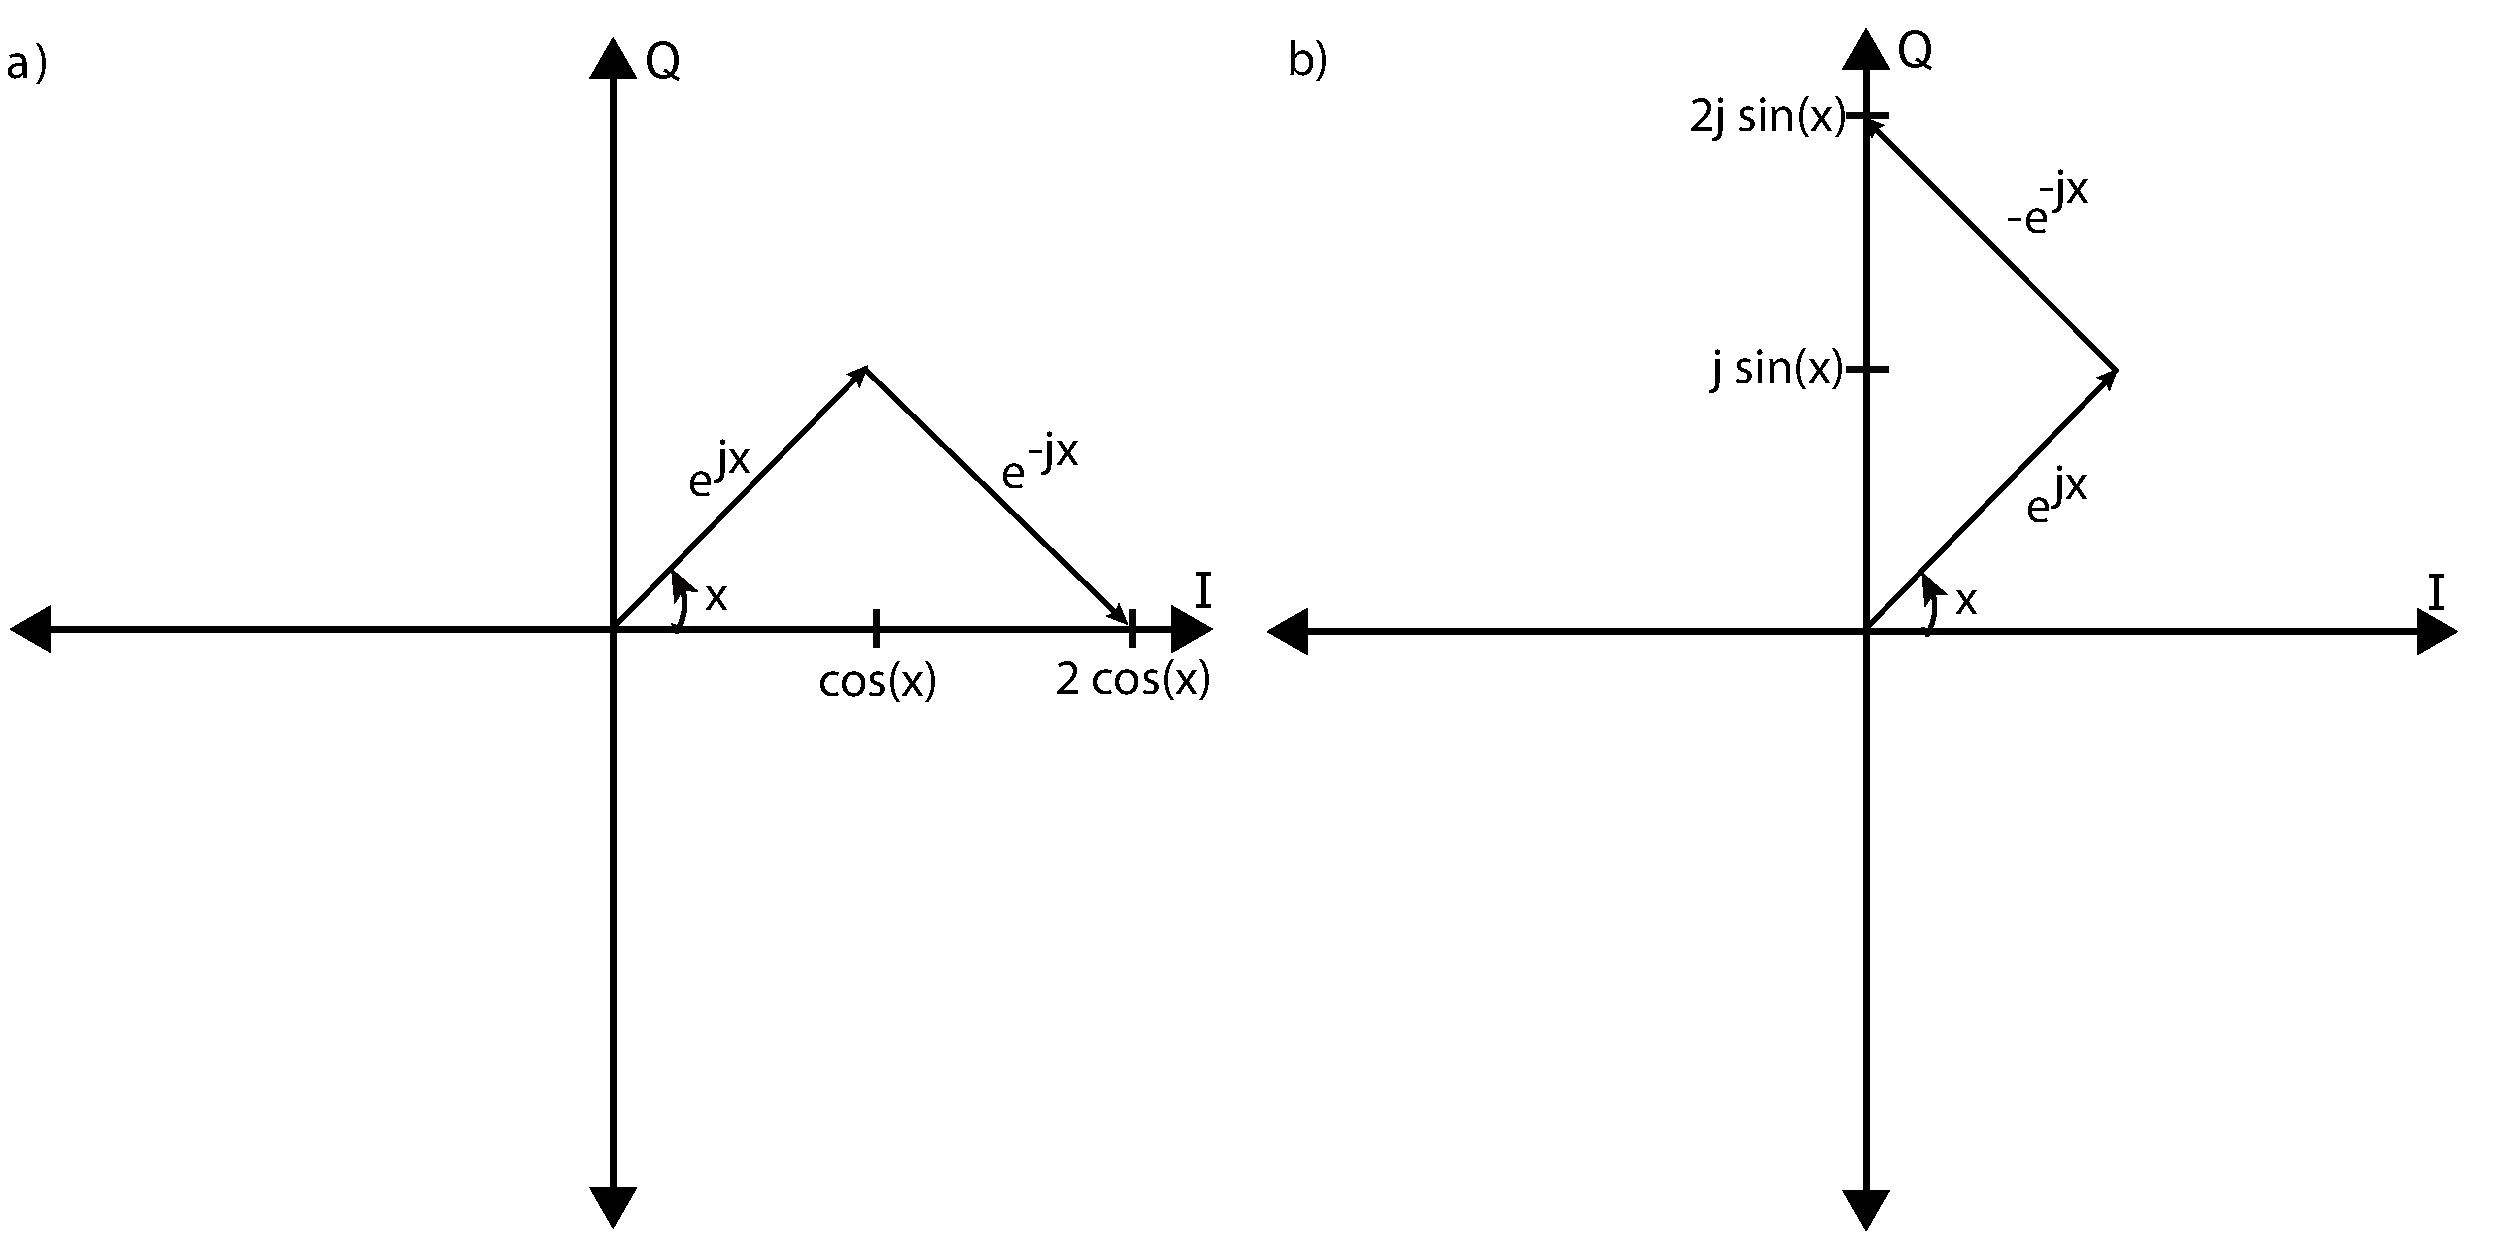
\includegraphics[width= \textwidth]{images/sin_cos_exp}
\caption{A visualization of the relationship between the cosine, sine, and the complex exponential. Part a) shows the sum of two complex vectors, $e^{jx}$ and $e^{-jx}$. The result of this summation lands exactly on the real axis with the value $2 \cos (x)$. Part b) shows a similar summation except this time summing the vectors $e^{jx}$ and $-e^{-jx}$. This summation lands on the imaginary axis with the value $2 \sin (x)$.}
\label{fig:sin_cos_exp}
\end{figure}


Both of these relationships can be visualized as vectors in the complex plane as shown in Figure \ref{fig:sin_cos_exp}. Part a) shows the cosine derivation. Here we add the two complex vectors $e^{jx}$ and $e^{-jx}$. Note that the sum of these two vectors results in a vector on the real (in-phase or I) axis. The magnitude of that vector is $2 \cos(x)$. Thus, by dividing the sum of these two complex exponentials by $2$, we get the value $\cos (x)$ as shown in Equation \ref{eq:cos_exp}.  Figure \ref{fig:sin_cos_exp} b) shows the similar derivation for sine. Here we are adding the complex vectors $e^{jx}$ and $-e^{-jx}$. The result of this is a vector on the imaginary (quadrature or Q) axis with a magnitude of $2 \sin (x)$. Therefore, we must divide by $2j$ in order to get $\sin (x)$. Therefore, this validates the relationship as described in Equation \ref{eq:sin_exp}.


\section{\gls{dft} Background}
\label{sec:DFTbackground}

The previous section provided a mathematical foundation for the Fourier series, which works on signals that are continuous and periodic. The Discrete Fourier Transform requires {\it discrete} periodic signals. The \gls{dft} converts a finite number of equally spaced samples into a finite number of complex sinusoids. In other words, it converts a sampled function from one domain (most often the time domain) to the frequency domain. The frequencies of the complex sinusoids are integer multiples of the \term{fundamental frequency} which is defined as the frequency related to the sampling period of the input function. Perhaps the most important consequence of the discrete and periodic signal is that it can be represented by a finite set of numbers. Thus, a digital system can be used to implement the \gls{dft}.  

The \gls{dft} works on input functions that uses both real and complex numbers. Intuitively, it is easier to first understand how the real \gls{dft} works, so we will ignore complex numbers for the time being and start with real signals in order to gain ease into the mathematics a bit. 
\begin{aside}
A quick note on terminology: We use lower case function variables to denote signals in the time domain. Upper case function variables are signals in the frequency domain. We use $( )$ for continuous functions and $[ ]$ for discrete functions. For example, $f( )$ is a continuous time domain function and $F( )$ is its continuous frequency domain representation. Similarly $g[ ]$ is a discrete function in the time domain and $G[ ]$ is that function transformed into the frequency domain. 
\end{aside}

To start consider Figure \ref{fig:basic-DFT}. The figure shows on the left a real valued time domain signal $g[ ]$ with $N$ samples or points running from $0$ to $N-1$. The \gls{dft} is performed resulting in the frequency domain signals corresponding to the cosine and sine amplitudes for the various frequencies. These can be viewed as a complex number with the cosine amplitudes corresponding to the real value of the complex number and the sine amplitudes providing the imaginary portion of the complex number. There are $N/2 + 1$ cosine (real) and $N/2 + 1$ sine (imaginary) values. We will call this resulting complex valued frequency domain function $G[ ]$. Note that the number of samples in frequency domain ($N/2 + 1$) is due to the fact that we are considering a real valued time domain signal; a complex valued time domain signal results in a frequency domain signal with $N$ samples.

\begin{figure}
\centering
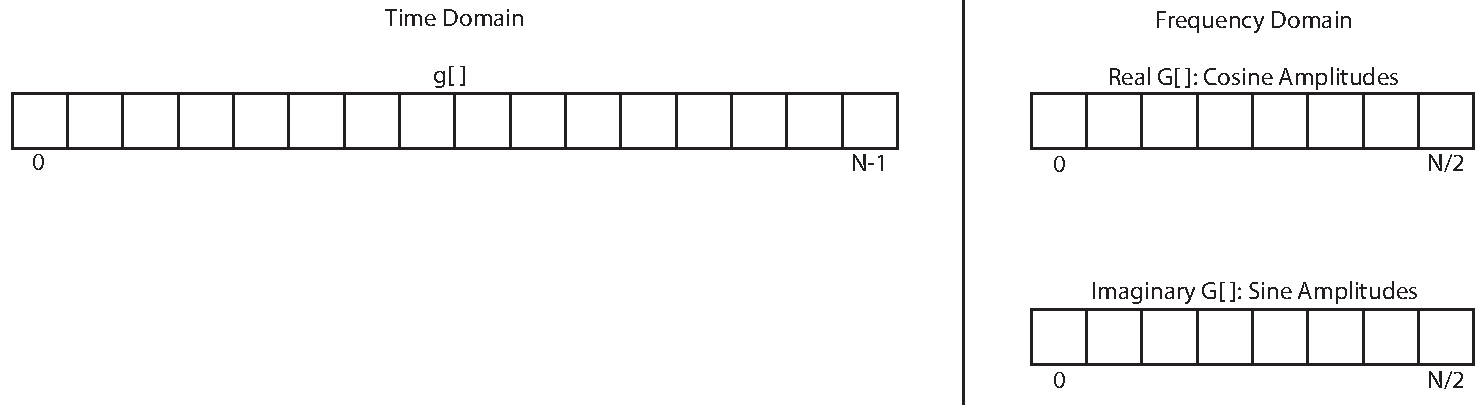
\includegraphics[width=\textwidth]{images/basic-DFT}
\caption{ A real valued discrete function $g[ ]$ in the time domain with $N$ points has a frequency domain representation with $N/2 + 1$ samples. Each of these frequency domain samples has one cosine and one sine amplitude value. Collectively these two amplitude values can be represented by a complex number with the cosine amplitude representing the real part and the sine amplitude the imaginary part. }
\label{fig:basic-DFT}
\end{figure}



An $N$ point \gls{dft} can be determined through a $N \times N$ matrix multiplied by a vector of size $N$, $G = S \cdot g$ where
\begin{equation}
S =
 \begin{bmatrix}
 \label{eq:Smatrix}
  1 & 1 & 1 & \cdots & 1 \\
  1 & s & s^2 & \cdots & s^{N-1} \\
  1 & s^2 & s^4 & \cdots & s^{2(N-1)} \\
  1 & s^3 & s^6 & \cdots & s^{3(N-1)} \\
  \vdots  & \vdots  & \vdots &\ddots & \vdots  \\
  1 & s^{N-1} & s^{2(N-1)}&\cdots & s^{(N-1)(N-1)}
 \end{bmatrix}
\end{equation} and $s = e^{\frac{-j 2 \pi}{N}}$.   Thus the samples in frequency domain are derived as 
\begin{equation}
G[k] = \displaystyle\sum\limits_{n=0}^{N-1} g[n] s^{kn} \text{ for } k = 0,\dots, N-1
\end{equation}
Figure \ref{fig:dft_visualization} provides a visualization of the \gls{dft} coefficients for an 8 point \gls{dft} operation. The eight frequency domain samples are derived by multiplying the 8 time domain samples with the corresponding rows of the $S$ matrix. Row 0 of the $S$ matrix corresponds to the DC component which is proportional to the average of the time domain samples. Multiplying Row 1 of the $S$ matrix with $g$ provides the cosine and sine amplitudes values for when there is one rotation around the unit circle. Since this is an 8 point \gls{dft}, this means that each phasor is offset by $45^{\circ}$. Performing eight $45^{\circ}$ rotations does one full rotation around the unit circle. Row 2 is similar except it performs two complete rotations around the unit circle, i.e., each individual rotation is $90^{\circ}$. This corresponds to a higher frequency. Row 3 does three complete rotations; Row 4 four rotations and so on. Each of these row times column multiplications gives the appropriate frequency domain sample. 

\begin{figure}
\centering
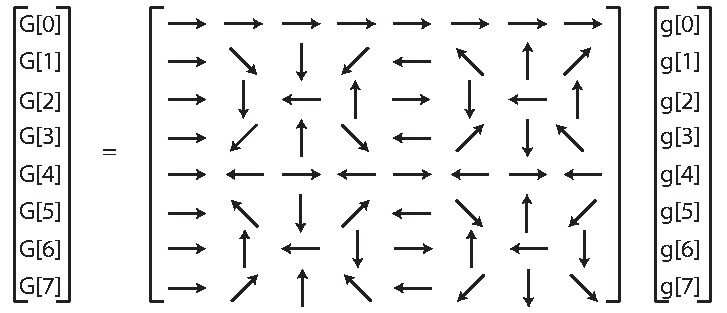
\includegraphics[width= 0.8 \textwidth]{images/dft-visualization}
\caption{ The elements of the $S$ shown as a complex vectors.  }
\label{fig:dft_visualization}
\end{figure}

Notice that the $S$ matrix is diagonally symmetric, that is $S[i][j] = S[j][i]$.  In addition, $S[i][j] = s^i*s^j = s^{(i+j)}$.  There is also interesting symmetry around Row 4. The phasors in Rows 3 and 5 are complex conjugates of each other, i.e., $S[3][j] = S[5][j]^*$. Similarly, Rows 2 and 6 ($S[2][j] = S[6][j]^*$), and Rows 1 and 7 ($S[1][j] = S[7][j]^*$) are each related by the complex conjugate operation. It is for this reason that the \gls{dft} of a real valued input signal with $N$ samples has only $N/2 + 1$ cosine and sine values in the frequency domain. The remaining $N/2$ frequency domain values provide redundant information so they are not needed. However, this is not true when the input signal is complex. In this case, the frequency domain will have $N + 1$ cosine and sine values. 

\section{Matrix-Vector Multiplication Optimizations}
\label{subsec:mvmul_implementation}

%\note{make sure this part is integrated. It was recently moved here}
Matrix-vector multiplication is the core computation of a \gls{dft}.  The input time domain vector is multiplied by a matrix with fixed special values. The result is a vector that corresponds to the frequency domain representation of the input time domain signal.  

In this section, we look at the hardware implementation of matrix-vector multiplication. We break this operation down into its most basic form (see Figure \ref{fig:matrix_vector_base}). This allows us to better focus the discussion on the optimizations rather than deal with all the complexities of using functionally correct \gls{dft} code. We will build a \gls{dft} core in the next section. 

\begin{figure}
\lstinputlisting{examples/matrix_vector_base.c}
\caption{Simple code implementing a matrix-vector multiplication.}\label{fig:matrix_vector_base}
\end{figure}

The code in Figure \ref{fig:matrix_vector_base} provides an initial starting point for synthesizing this operation into hardware. We use a custom data type called \lstinline|BaseType| that is currently mapped as a \lstinline|float|. This may seem superfluous at the time, but this will allow us in the future to easily experiment with different number representations for our variables (e.g., signed or unsigned fixed point with different precision). The \lstinline|matrix_vector| function has three arguments. The first two arguments \lstinline|BaseType M[SIZE][SIZE]| and \lstinline|BaseType V_In[SIZE]| are the input matrix and vector to be multiplied. The third argument \lstinline|BaseType V_Out[SIZE]| is the resultant vector. By setting \lstinline|M = S|  and \lstinline|V_In| to a sampled time domain signal, the \lstinline|V_Out| will contain the \gls{dft}. \lstinline|SIZE| is a constant that determines the number of samples in the input signal and correspondingly the size of the \gls{dft}.

The algorithm itself is simply a nested \lstinline|for| loop. The inner loop (\lstinline|dot_product_loop|) computes the \gls{dft} coefficients starting from \lstinline|0| and going to \lstinline|SIZE - 1|. However, this relatively simple code has many design choices that can be performed when mapping to hardware. 

Whenever you perform HLS, you should think about the architecture that you wish to synthesize. Memory organization is one of the more important decisions. The question boils down to \emph{where do you store the data from your code?} There are a number of options when mapping variables to hardware. The variable could simply be a set of wires (if its value never needs saved across a cycle), a register, RAM or FIFO. All of these options provide tradeoffs between performance and area. 

Another major factor is the amount of parallelism that is available within the code. Purely sequential code has few options for implementation. On the other hand, code with a significant amount of parallelism has implementation options that range from purely sequentially to fully parallel. These options obviously have different area and performance. We will look at how both memory configurations and parallelism effect the hardware implementation for the matrix-vector implementation of the \gls{dft}.

\begin{figure}
\centering
%\includesvg{images/matrix_vector_sequential}
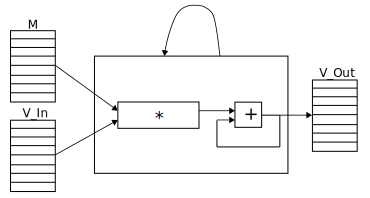
\includegraphics[width= 0.4 \textwidth]{images/matrix_vector_sequential}
\includesvg{dft_behavior_loop_sequential}
\caption{A possible implementation of matrix-vector multiplication from the code in Figure \ref{fig:matrix_vector_base}.}
\label{fig:matrix_vector_sequential}
\end{figure}

Figure \ref{fig:matrix_vector_sequential} shows a sequential architecture for matrix-vector multiplication with one multiply and one addition operator.  Logic is created to access the \lstinline|V_In| and \lstinline|M| arrays which are stored in BRAMs. Each element of \lstinline|V_Out| is computed and stored into the BRAM. This architecture is essentially what will result from synthesizing the code from Figure \ref{fig:matrix_vector_base} with no directives. It does not consume a lot of area, but the task latency and task interval are relatively large.

\section{Pipelining and Parallelism}

There is substantial opportunity to exploit parallelism in the matrix-multiplication example. We start by focusing on the inner loop. The expression \lstinline|sum += V_In[j] * M[i][j];| is executed in each iteration of the loop. The variable \lstinline|sum|, which is keeping a running tally of the multiplications, is being reused in each iteration and takes on a new value. This inner loop can be rewritten as shown Figure \ref{fig:matrix_vector_base_unroll_inner}.  In this case, the sum variable has been completely eliminated and replaced with multiple intermediate values in the larger expression.

\begin{figure}
\lstinputlisting{examples/matrix_vector_base_unroll_inner.c}
\caption{The matrix-vector multiplication example with a manually unrolled inner loop.}
\label{fig:matrix_vector_base_unroll_inner}
\end{figure}


\begin{aside}
Loop unrolling is performed automatically by \VHLS in a pipelined context.  Loop unrolling can also be requested by using \lstinline|#pragma HLS unroll| or the equivalent directive outside of a pipelined context.  
\end{aside} 

It should be clear that the new expression replacing the inner loop has significant amount of parallelism. Each one of the multiplications can be performed simultaneously, and the summation can be performed using an adder tree. The data flow graph of this computation is shown in Figure \ref{fig:matrix_vector_unroll_inner_dfg}. 

\begin{figure}
\centering
\includesvg{matrix_vector_unroll_inner}
%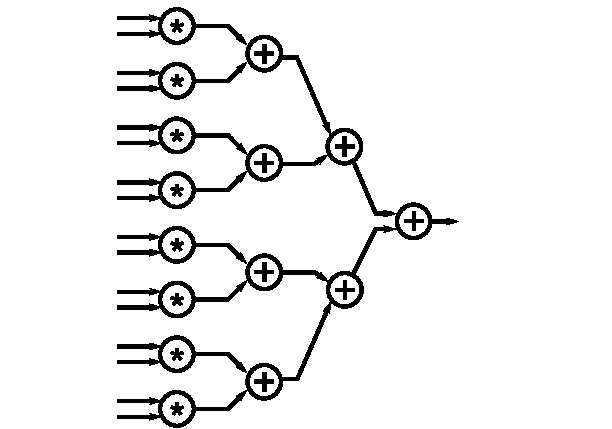
\includegraphics[width=.8\textwidth]{images/matrix_vector_unroll_inner.pdf}
\caption{A data flow graph of the expression resulting from the unrolled inner loop from Figure \ref{fig:matrix_vector_base_unroll_inner}.}\label{fig:matrix_vector_unroll_inner_dfg}
\end{figure}

If we wish to achieve the minimum task latency for the expression resulting from the unrolled inner loop, all eight of the multiplications should be executed in parallel. Assuming that the multiplication has a latency of 3 cycles and addition has a latency of 1 cycle, then all of the \lstinline|V_In[j] * M[i][j]| operations are completed by the third time step. The summation of these eight intermediate results using an adder tree takes $\log 8 = 3$ cycles. Hence, the body of \lstinline|data_loop| now has a latency of 6 cycles for each iteration and requires 8 multipliers and 7 adders.  This behavior is shown in the left side of  Figure \ref{fig:dft_behavior1}.  Note that the adders could be reused across Cycle 4-6, which would reduce the number of adders to 4. However, adders are typically not shared when targeting FPGAs since an adder and a multiplexer require the same amount of FPGA resources (approximately 1 LUT per bit for a 2-input operator). 

\begin{figure}
\centering
\includesvg{dft_behavior1}
%\includesvg{dft_behavior2}
\caption{Possible sequential implementations resulting from the unrolled inner loop from Figure \ref{fig:matrix_vector_base_unroll_inner}.}\label{fig:dft_behavior1}
\end{figure}

If we are not willing to use 8 multipliers, there is an opportunity to reduce resource usage in exchange for increasing the number of cycles to execute the function. For example, using 4 multipliers would result in a latency of 6 cycles for the multiplication of the eight \lstinline|V_In[j] * M[i][j]| operations, and an overall latency of 9 cycles to finish the body of \lstinline|data_loop|. This behavior is shown in the right side of Figure \ref{fig:dft_behavior1}.  You could even use fewer multipliers at the cost of taking more cycles to complete the inner loop.

Looking at Figure \ref{fig:dft_behavior1}, it is apparent that there are significant periods where the operators are not performing useful work, reducing the overall efficiency of the design.  It would be nice if we could reduce these periods.  In this case we can observe that each iteration of \lstinline|data_loop| is, in fact completely independent, which means that they can be executed concurrently.  Just as we unrolled \lstinline{dot_product_loop}, it's also possible to unroll \lstinline{data_loop} and perform all of the multiplications concurrently.  However, this would require a very large amount of FPGA resources.  A better choice is to enable each iteration of the loop to start as soon as possible, while the previous execution of the loop is still executing.  This process is called \gls{looppipelining} and is achieved in \VHLS using \lstinline|#pragma HLS pipeline|.  In most cases, loop pipelining reduces the interval of a loop to be reduced, but does not affect the latency.  Loop pipelined behavior of this design is shown in Figure \ref{fig:dft_behavior2}. 

\begin{figure}
\centering
\includesvg{dft_behavior2}
\caption{Possible pipelined implementations resulting from the unrolled inner loop from Figure \ref{fig:matrix_vector_base_unroll_inner}.}\label{fig:dft_behavior2}
\end{figure}

Until now, we have only focused on operator latency.  It is common to have pipelined functional units; most functional units in \VHLS are fully pipelined with an interval of one. Even though it might take 3 cycles for a single multiply operation to complete, a new multiply operation could start every clock cycle on a pipelined multiplier.  In this way, a single functional unit may be able to simultaneously execute many multiply operations at the same time.  For instance, a multiplier with a latency of 3 and an interval of 1 could be simultaneously executing three multiply operations. 

By taking advantage of pipelined multipliers, we can reduce the latency of the unrolled inner loop without adding additional operators.  One possible implementation using three pipelined multipliers is shown on the left in Figure \ref{fig:dft_behavior_pipelined}.  In this case, the multiplication operations can execute concurrently (because they have no data dependencies), while the addition operations cannot begin until the first multiplication has completed.  In the figure on the right, a pipelined version of this design is shown, with an interval of 3, which is similar to the results of \VHLS if \lstinline|#pragma  HLS pipeline II=3| is applied to the \lstinline|data_loop|.  In this case, not only are individual operations executing concurrently on the same operators, but those operations may come from different iterations of \lstinline|data_loop|.  

\begin{figure}
\centering
\includesvg{dft_behavior3}
\caption{Possible implementations resulting from the unrolled inner loop from Figure \ref{fig:matrix_vector_base_unroll_inner} using pipelined multipliers.}\label{fig:dft_behavior_pipelined}
\end{figure}

At this point you may have observed that pipelining is possible at different levels of hierarchy, including the operator level, loop level, and function level.  Furthermore, pipelining at different levels are largely independent!  We can use pipelined operators in a sequential loop, or we can use sequential operators to build a pipelined loop.  It's also possible to build pipelined implementations of large functions which can be shared in \VHLS just like primitive operators.  In the end, what matters most is how many operators are being instantiated, their individual costs, and how often they are used.

%By taking advantage of this pipelined multiplier, we can reduce the latency of the unrolled inner loop without adding additional operators. Figure \ref{fig:matrix_vector_unroll_inner_dfg_pipelined} shows the unrolled inner loop using a three stage pipelined multiplier. Here the first three multiply operations (corresponding to the operations \texttt{V\_In[0] * M[i][0], V\_In[1] * M[i][1], V\_In[2] * M[i][2] , V\_In[3] * M[i][3]}) can use the same multiplier. Note that this multiplier can only start one multiply operation in any clock cycle, and the operations still requires 3 cycles to complete. Likewise the operations \texttt{V\_In[4] * M[i][4], V\_In[5] * M[i][5], V\_In[6] * M[i][6] , V\_In[7] * M[i][7]} can use the same multiplier. Thus only 2 multipliers are required. 

%\begin{figure}
%\centering
%\includesvg{images/matrix_vector_unroll_inner}
%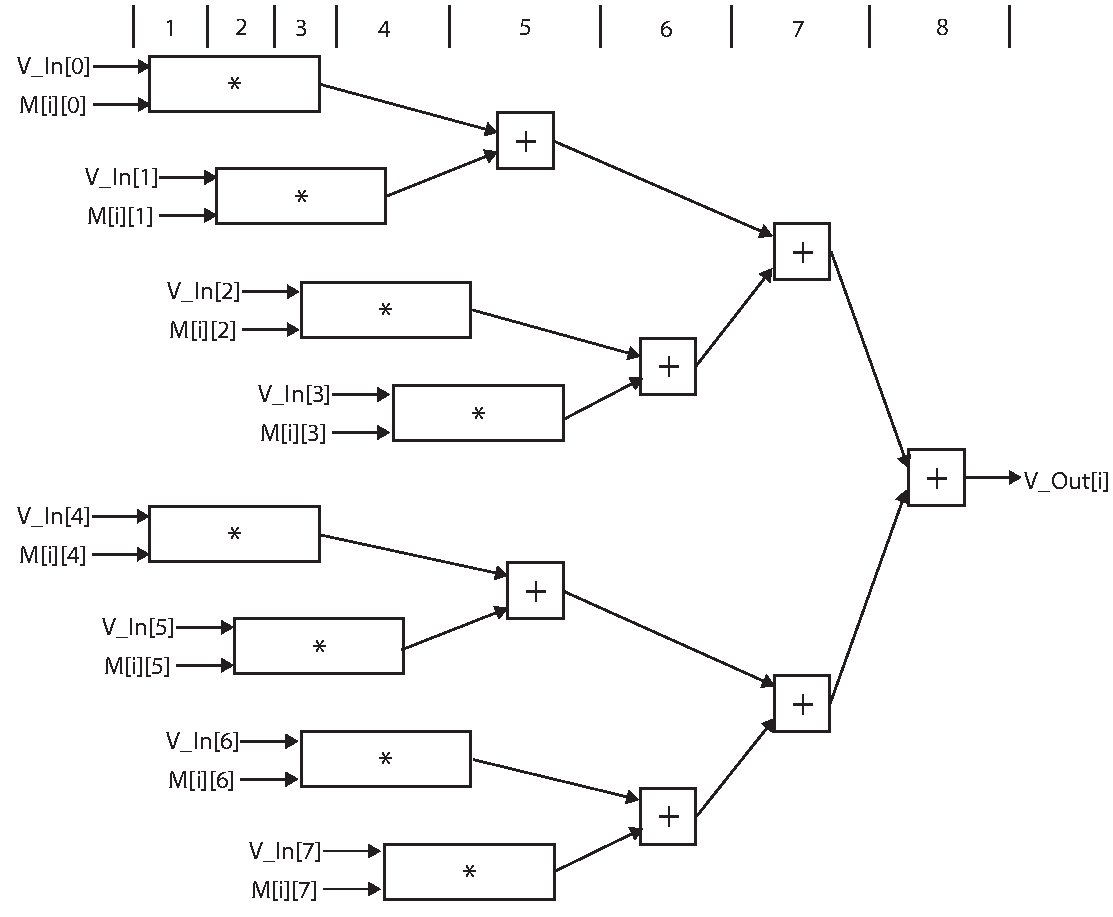
\includegraphics[width=\textwidth]{images/matrix_vector_unroll_inner_pipelined.pdf}
%\caption{A data flow graph of the expression resulting from the unrolled inner loop from Figure \ref{fig:matrix_vector_base_unroll_inner} using pipelined multipliers.}\label{fig:matrix_vector_unroll_inner_dfg_pipelined}
%\marginnote{This needs a way to show the mapping of operation -> operator}
%\end{figure}

\section{Storage Tradeoffs and Array Partitioning}
\label{subsec:dft_array_partitioning}

Up until this point, we have assumed that the data in arrays (\lstinline|V_In[]|, \lstinline|M[][]|, and \lstinline|V_Out[]| are accessible at anytime.  In practice, however, the placement of the data plays a crucial role in the performance and resource usage. In most processor systems, the memory architecture is fixed and we can only adapt the program to attempt to best make use of the available memory hierarchy, taking care to minimize register spills and cache misses, for instance.  In HLS designs, we can also explore and leverage different memory structures and often try to find the memory structure that best matches a particular algorithm.  Typically large amounts of data are stored in off-chip memory, such as DRAM, flash, or even network-attached storage. However, data access times are typically long, on the order of tens to hundreds (or more) of cycles. Off-chip storage also relatively large amounts of energy to access, because large amounts of current must flow through long wires.  On-chip storage, in contrast can be accessed quickly and is much lower power.  I contrast it is more limited in the amount of data that can be stored.  A common pattern is to load data into on-chip memory in a block, where it can then be operated on repeatedly.  This is similar to the effect of caches in the memory hierarchy of general purpose CPUs.

The primary choices for on-chip storage on in embedded memories (e.g., block RAMs) or in flip-flops (FFs). These two options have their own tradeoffs. Flip-flop based memories allow for multiple reads at different addresses in a single clock.  It is also possible to read, modify, and write a Flip-flop based memory in a single clock cycle.  However, the number of FFs is typically limited to around 100 Kbytes, even in the largest devices. In practice, most flip-flop based memories should be much smaller in order to make effective use of other FPGA resources.  Block RAMs (BRAMs) offer higher capacity, on the order Mbytes of storage, at the cost of limited accessibility. For example, a single BRAM can store more than 1-4 Kbytes of data, but access to that data is limited to two different addresses each clock cycle. Furthermore, BRAMs are required to have a minimum amount of pipelining (i.e. the read operation must have a latency of at least one cycle).  Therefore, the fundamental tradeoff boils down to the required bandwidth versus the capacity. 

If throughput is the number one concern, all of the data would be stored in FFs. This would allow any element to be accessed as many times as it is needed each clock cycle. However, as the size of arrays grows large, this is not feasible.  In the case of matrix-vector multiplication, storing a 1024 by 1024 matrix of 32-bit integers would require about 4 MBytes of memory.   Even using BRAM, this storage would require about 1024 BRAM blocks, since each BRAM stores around 4KBytes.  On the other hand, using a single large BRAM-based memory means that we can only access two elements at a time.  This obviously prevents higher performance implementations, such as in Figure \ref{fig:matrix_vector_unroll_inner_dfg}, which require accessing multiple array elements each clock cycle (all eight elements of \lstinline|V_In[]| along with 8 elements of \lstinline|M[][]|).  In practice, most designs require larger arrays to be strategically divided into smaller BRAM memories, a process called \gls{arraypartitioning}.  Smaller arrays (often used for indexing into larger arrays) can be partitioned completely into individual scalar variables and mapped into FFs.  Matching pipelining choices and array partitioning to maximize the efficiency of operator usage and memory usage is an important aspect of design space exploration in HLS.

\begin{aside}
\VHLS will perform some array partitioning automatically, but as array partitioning tends to be rather design-specific it is often necessary to guide the tool for best results.  Global configuration of array partitioning is available in the \lstinline|config_array_partition| project option.  Individual arrays can be explicitly partitioned using the \lstinline|array_partition| directive. The directive \lstinline|array_partition complete| will split each element of an array into its own register, resulting in a flip-flop based memory.  As with many other directive-based optimizations, the same result can also be achieved by rewriting the code manually.  In general, it is preferred to use the tool directives since it avoids introducing bugs and keeps the code easy to maintain.
\end{aside}

%The question then becomes how do we store the data across these different BRAMs. For example, we could store the $M$ matrix in row-major or column-major order. This may effect the performance depending upon the data access patterns. For example, if we could partition the data in such a way that none of the accesses at any time occur to the same BRAM, then this would allow for all of the memory access operations to be scheduled at the same cycle. However, if the data was partitioned such that the data accesses all went to the same BRAM at any given time, these access must be sequentialized since the BRAM only has a limited number of read ports. Therefore, it is important to carefully consider how the data access patterns required by the code when you are partitioning your data.

%\begin{aside}
%Row-major order stores the values of an array with the elements in a row in consecutive order. For example the matrix when stored in row-major order is 
%\[
%  \begin{bmatrix}
%   1 & 2 & 3 \\
%   4 & 5 & 6\\
%   7 & 8 & 9\\
%  \end{bmatrix}
%= \begin{bmatrix} 1 & 2 & 3 & 4 & 5 & 6 & 7 & 8 & 9\\
%\end{bmatrix}
%\] The same matrix in column-major order is 
%\[ 
%	\begin{bmatrix} 1 & 4 & 7 & 2 & 5 & 8 & 3 & 6 & 9\\ \end{bmatrix} \]
%\end{aside}

Returning to the matrix-vector multiplication code in Figure \ref{fig:matrix_vector_base}, we can achieve a highly parallel implementation with the addition of only a few directives, as shown in Figure \ref{fig:matrix_vector_optimized}.  The resulting architecture is shown in Figure \ref{fig:matrix_vector_optimized_behavior}.  Notice that the inner \lstinline|j| loop is automatically unrolled by \VHLS and hence every use of \lstinline|j| is replaced with constants in the implementation.   This design demonstrates the most common use of array partitioning where the array dimensions that are partitioned (in this case, \lstinline|V_In[]| and the second dimension of \lstinline|M[][]|) are indexed with the constants (in this case the loop index \lstinline|j| of the unrolled loop).  This enables an architecture where multiplexers are not required to access the partitioned arrays.

\begin{figure}
\lstinputlisting{examples/matrix_vector_optimized.c}
\caption{Matrix-vector multiplication with a particular choice of array partitioning and pipelining. }
\label{fig:matrix_vector_optimized}
\end{figure}

\begin{figure}
\includesvg{matrix_vector_optimized}
\caption{Matrix-vector multiplication architecture with a particular choice of array partitioning and pipelining.  The pipelining registers have been elided and the behavior is shown at right.}
\label{fig:matrix_vector_optimized_behavior}
\end{figure}

It's also possible to achieve other designs which use fewer multipliers and have lower performance.   For instance, in Figure \ref{fig:dft_behavior_pipelined}, these designs use only three multipliers, hence we only need to read three elements of matrix \lstinline|M[][]| and vector \lstinline|V_in[]| each clock cycle. Completely partitioning these arrays would result in extra multiplexing as shown in Figure \ref{fig:matrix_vector_partition_factor}.  In actuality the arrays only need to be partitioned into three physical memories.  Again, this partitioning could be implemented manually by rewriting code or in \VHLS using the \lstinline|array_partition cyclic| directive.

\begin{aside}
Beginning with an array \lstinline|x| containing the values \[ 
\begin{bmatrix} 
1 & 2 & 3 & 4 & 5 & 6 & 7 & 8 & 9\\
\end{bmatrix}
\]
The directive \lstinline{array_partition variable=x factor=2 cyclic} on the array would split it into two arrays which are 
\[\begin{bmatrix}
1 & 3 & 5 & 7 & 9\\
\end{bmatrix} \text{and} 
\begin{bmatrix}
2 & 4 & 6 & 8 \\
\end{bmatrix}
\]
Similarly, the directive \lstinline{array_partition variable=x factor=2 block} would split it into two arrays
\[\begin{bmatrix}
1 & 2 & 3 & 4 & 5\\
\end{bmatrix} \text{and} 
\begin{bmatrix}
6 & 7 & 8 & 9 \\
\end{bmatrix}
\]
\end{aside}

\begin{figure}
\includesvg{matrix_vector_partition_factor}
\caption{Matrix-vector multiplication architectures at II=3 with a particular choices of array partitioning.  On the left, the arrays have been partitioned more than necessary, resulting in multiplexers.  On the right, the arrays are partitioned with factor=3. In this case, multiplexing has been reduced, but the \lstinline|j| loop index becomes a part of the address computations.}
\label{fig:matrix_vector_partition_factor}
\end{figure}

\begin{exercise}
Study the effects of varying pipeline II and array partitioning on the performance and area. Plot the performance in terms of number of matrix vector multiply operations per second (throughput) versus the unroll and array partitioning factor. Plot the same trend for area (showing LUTs, FFs, DSP blocks, BRAMs). What is the general trend in both cases? Which design would you select? Why?
\end{exercise} 

Alternatively, similar results can be achieved by pipelining and applying \gls{partial_loop_unrolling} to the inner \lstinline|dot_product_loop|.   Figure \ref{fig:matrix_vector_unroll_inner2} shows the result of unrolling the inner loop of the matrix-vector multiplication code by a factor of 2. You can see that the loop bounds now increment by 2. Each loop iteration requires 2 elements of matrix \lstinline|M[][]| and vector \lstinline|V_in[]| each iteration and perform two multiplies instead of one. In this case after loop unrolling \VHLS can implement the operations in both expressions in parallel, corresponding to two iterations of the original loop. Note that without appropriate array partitioning, unrolling the inner loop may offer no increase in performance, as the number of concurrent read operations is limited by the number of ports to the memory.  In this case, we can store the data from the even columns in one BRAM and the data from the odd columns in the other. This is due to the fact that the unrolled loop is always performing one even iteration and one odd iteration. 

\begin{aside}
The HLS tool can automatically unroll loops using the \texttt{unroll} directive. The directive takes a \texttt{factor} argument which is a positive integer denoting the number of times that the loop body should be unrolled. 
\end{aside}

\begin{figure}
\lstinputlisting{examples/matrix_vector_unroll_inner2.c}
\caption{The inner loop of matrix-vector multiply manually unrolled by a factor of two. }
\label{fig:matrix_vector_unroll_inner2}
\end{figure}

\begin{exercise}
Manually divide \lstinline|M[][]| and vector \lstinline|V_in[]| into separate arrays in the same manner as the directive \lstinline|array_partition cyclic factor=2|. How do you have to modify the code in order to change the access patterns? Now manually unroll the loop by a factor of two. How do the performance results vary between the original code (no array partitioning and no unrolling), only performing array partitioning, and performing array partitioning and loop unrolling? Finally, use the directives to perform array partitioning and loop unrolling. How do those results compare to your manual results?
\end{exercise} 

In this code, we see that array partitioning often goes hand in hand with our choices of pipelining. Array partitioning by a factor of 2 enables an increase in performance by a factor of 2, which can be achieved either by partially unrolling the inner loop by a factor of 2 or by reducing the II of the outer loop by a factor of 2.  Increasing performance requires a corresponding amount of array partitioning.  In the case of matrix vector multiplication, this relationship is relatively straightforward since there is only one access to each variable in the inner loop.  In other code, the relationship might be more complicated.  Regardless, the goal of a designer is usually to ensure that the instantiated FPGA resources are used efficiently.  Increasing performance by a factor of 2 should use approximately twice as many resources.  Decreasing performance by a factor of 2 should use approximately half as many resources.

\begin{exercise}
Study the effects of loop unrolling and array partitioning on the performance and area. Plot the performance in terms of number of matrix vector multiply operations per second (throughput) versus the unroll and array partitioning factor. Plot the same trend for area (showing LUTs, FFs, DSP blocks, BRAMs). What is the general trend in both cases? Which design would you select? Why?
\end{exercise} 


\section{Baseline Implementation}
\label{subsec:dft_implementation}

We just discussed some optimizations for matrix-vector multiplication. This is a core computation in performing a \gls{dft}. However, there are some additionally intricacies that we must consider to move from the matrix-vector multiplication in the previous section to a functionally complete \gls{dft} hardware implementation. We move our focus to the \gls{dft} in this section, and describe how to optimize it to make it execute most efficiently.  

One significant change that is required is that we must be able to handle complex numbers.  As noted in Section \ref{sec:DFTbackground} because the elements of the $S$ matrix are complex numbers, the \gls{dft} of a real-valued signal is almost always a complex-valued signal.   It is also common to perform the \gls{dft} of a complex-valued signal, to produce a complex-valued result.  Additionally, we need to handle fractional or possibly floating point data, rather than integers.  This can increase the cost of the implementation, particularly if floating point operations need to be performed.  In addition, floating point operators, particularly addition, have much larger latency than integer addition.  This can make it more difficult to achieve II=1 loops.  A second change is that we'd like to be able to scale our design up to large input vector sizes, perhaps N=1024 input samples.  Unfortunately, if we directly use matrix-vector multiplication, then we must store the entire $S$ matrix.  Since this matrix is the square of the input size, it becomes prohibitive to store for large input sizes.  In the following sections, we'll discuss techniques to address both of these complexities. 

As is typical when creating a hardware implementation using high level synthesis, we start with a straightforward or naive implementation. This provides us with a baseline code that we can insure has the correct functionality. Typically, this code runs in a very sequential manner; it is not highly optimized and therefore may not meet the desired performance metrics. However, it is a necessary step to insure that the designer understand the functionality of the algorithm, and it serves as starting point for future optimizations.

\begin{figure}
\lstinputlisting{examples/dft.c}
\caption{Baseline code for the \gls{dft}.}
\label{fig:dft_code}
\end{figure}

Figure \ref{fig:dft_code} shows a baseline implementation of the \gls{dft}. This uses a doubly nested \lstinline|for| loop. The inner loop multiplies one row of the $S$ matrix with the input signal. Instead of reading the $S$ matrix as an input, this code computes an element of $S$ in each each iteration of the inner loop, based on the current loop indices.  This phasor is converted to Cartesian coordinates (a real part and an imaginary part) using the \lstinline|cos()| and \lstinline|sin()| functions. The code then performs a complex multiplication of the phasor with the appropriate sample of the input signal and accumulates the result. After $N$ iterations of this inner loop, one for each column of $S$, one frequency domain sample is calculated. The outer loop also iterates $N$ times, once for each row of $S$.  As a result, the code computes an expression for \lstinline|w| $N$ times, but computes the \lstinline|cos()| and \lstinline|sin()| functions and a complex multiply-add $N^2$ times.

This code uses a function call to calculate \lstinline|cos()| and \lstinline|sin()| values. \VHLS is capable of synthesizing these functions using its built-in math library. There are several possible algorithms \cite{detrey07hotbm} for implementing trigonometric functions including CORDIC, covered in Chapter \ref{chapter:cordic}.  However, generating precise results for these functions can be expensive.  There are several possibilities for eliminating these function calls, since the inputs aren't arbitrary.  We will discuss these tradeoffs in more detail later.    A sequential implementation of this code is show in Figure \ref{fig:dft_sequential_arch}. 

%Remember, however, that the results of these $\sin()$ and $\cos()$ function calls are just the elements of $S$ and are only dependent on the constant $N$ and not the input data. This is often the case, e.g., you will know that you wish to do a 256 or 1024 point \gls{dft}. Therefore, it is possible to eliminate these $\cos()$ and $\sin()$ function calls by using a lookup table that holds the values of the $S$ matrix. This replaces the costly implementation of $\cos()$ and $\sin()$ with a memory access. The $S$ matrix can be stored in BRAMs for smaller size \gls{dft}. However, larger \gls{dft}s can quickly exhaust the available BRAM space on-chip. This provides one possible design tradeoff, which utilizes more memory in order to perform computation faster. We discuss this tradeoff in more detail later.

\begin{figure}
\centering
\includesvg{dft_behavior_baseline}
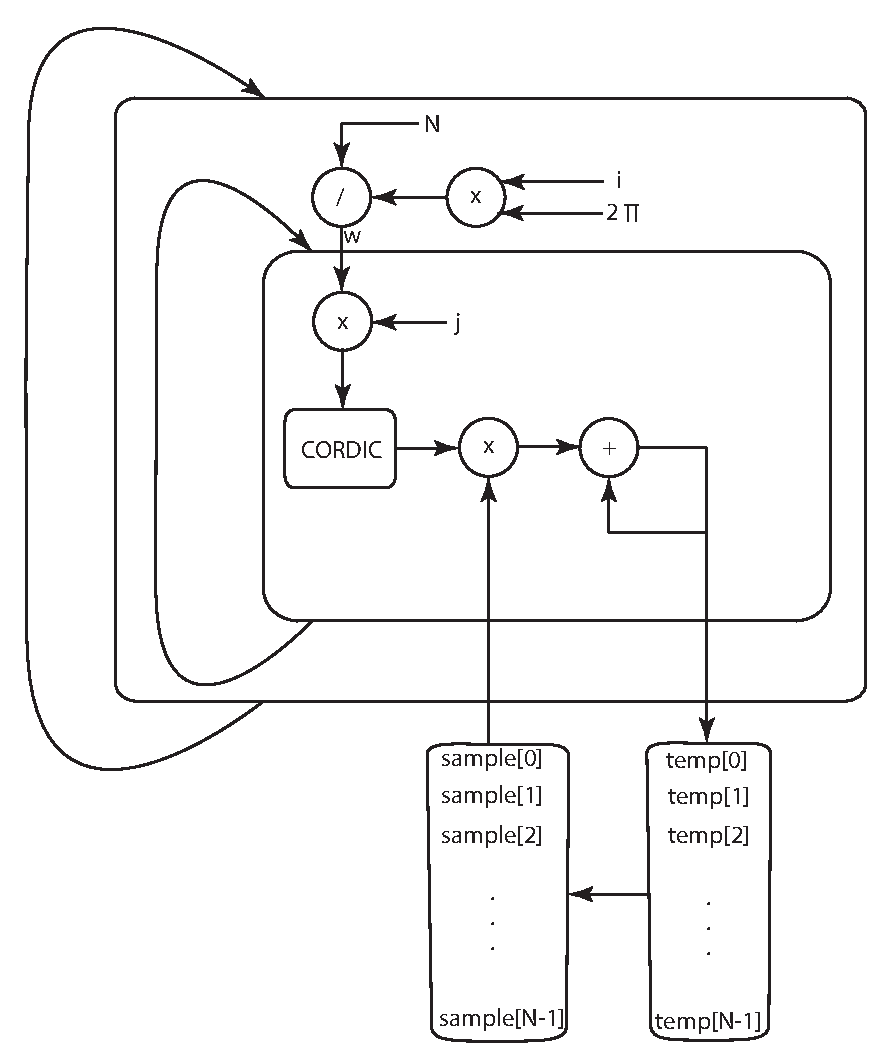
\includegraphics[width= 0.7 \textwidth]{images/dft_sequential_arch}
\caption{ A high level architectural diagram of the \gls{dft} as specified in the code from Figure \ref{fig:dft_code}. This is not a comprehensive view of the architecture, e.g., it is missing components related to updating the loop counters \lstinline|i| and \lstinline|j|. It is meant to provide an approximate notion of how this architecture will be synthesized.  Here we've assumed that floating point operators take 4 clock cycles.}
\label{fig:dft_sequential_arch}
\end{figure}

%Figure \ref{fig:dft_sequential_arch} provides an overview of the one potential \gls{dft} architecture. This hardware implementation is highly sequential. The data path corresponding to the inner loop is executed $N \times N$ times, which corresponds to $N^2$ computations of $\cos()$ and $\sin()$ and $N^2$ complex multiplications and additions.  In each iteration of the outer loop, the variable $w$ is computed. This is essentially determining the amount of rotation that each row of the $S$ matrix requires. The phasor angle is then calculated in each iteration of the inner loop through a multiplication by the loop iterator $j$. The result is fed into a CORDIC operator to determine the sine and cosine values used in the complex multiplication and subsequent summation.  The result of the inner loop is summed into the appropriate $temp[]$ variable. Finally, after these two nested loops are finished, the values in the $temp[]$ array are copied into the $sample[]$ array. This is called an in-place \gls{dft}, i.e., the output frequency samples are stored in the same location as the input signal samples. This saves memory at the expense of $N$ additional read and write operations. 

\begin{exercise}
What changes would this code require if you were to use a CORDIC that you designed, for example, from Chapter \ref{chapter:cordic}? Would changing the accuracy of the CORDIC core make the \gls{dft} hardware resource usage change? How would it effect the performance? 
\end{exercise}

\begin{exercise}
Implement the baseline code for the \gls{dft} using HLS.  Looking at the reports, what is the relative cost of the implementation of the trignometric functions, compared to multiplication and addition?  Which operations does it make more sense to try to optimize?  What performance can be achieved by pipelining the inner loop?
\end{exercise}

\section{\gls{dft} optimization}
\label{subsec:dft_optimization}

The baseline \gls{dft} implementation of the previous section uses relatively high precision \lstinline|double| datatypes.  Implementing floating point operations is typically very expensive and requires many pipeline stages, particularly for double precision.  We can see in Figure \ref{fig:dft_sequential_arch} that this significantly affects the performance of the loop.  With pipelining, the affect of these high-latency operations is less critical, since multiple executions of the loop can execute concurrently.  The exception in this code are the \lstinline|temp_real[]| and \lstinline|temp_imag[]| variables, which are used to accumulate the result.  This accumulation is a \gls{recurrence} and limits the achievable II in this design when pipelining the inner loop.   This operator dependence is shown in Figure \ref{fig:dft_recurrence_behavior}.

\begin{figure}
\centering
\includesvg{dft_recurrence_behavior}
\caption{Pipelined version of the behavior in Figure \ref{fig:dft_sequential_arch}.  In this case, the initiation interval of the loop is limited to 4, since each floating point addition takes 4 clock cycles to complete and the result is required before the next loop iteration begins (the dependence shown in red).  The dependencies  for all iterations are summarized in the diagram on the right.}
\label{fig:dft_recurrence_behavior}
\end{figure}

One possible solution is to reduce the precision of the computation.  This is always a valuable technique when it can be applied, since it reduces the resources required for each operation, the memory required to store any values, and often reduces the latency of operations as well.  For instance we could use the 32-bit \lstinline|float| type or the 16-bit \lstinline|half| types rather than double.  Many signal processing systems avoid floating point data types entirely and use fixed point data types\ref{sec:number_representation}.  For commonly used integer and fixed-point precisions, each addition can be completed in a single cycle, enabling the loop to be pipelined at II=1.

\begin{exercise}
What happens to the synthesis result of the code in Figure \ref{fig:dft_code} if you change all of the data types from $double$ to $float$? Or from $double$ to $half$? Or to a fixed point value? How does this change the performance (interval and latency) and the resource usage? Does it change the values of the output frequency domain samples?
\end{exercise}

A more general solution to achieve II=1 with floating point accumulations is to process the data in a different order.  Looking at Figure \ref{fig:dft_recurrence_behavior} we see that the recurrence exists (represented by the arrow) because the \lstinline|j| loop is the inner loop.  If the inner loop were the \lstinline|i| loop instead, then we wouldn't need the result of the accumulation before the next iteration starts.  We can achieve this in the code by interchanging the order of the two loops.  This optimization is often called \gls{loopinterchange} or pipeline-interleaved processing\cite{lee87sdfArchitecture}.  In this case, it may not be obvious that we can rearrange the loops because of the extra code inside the outer \lstinline|i| loop.  Fortunately, the $S$ matrix is diagonally symmetric, and hence \lstinline|i| and \lstinline|j| can be exchanged in the computation of \lstinline|w|.  The result is that we can now achieve an II of 1 for the inner loop.  The tradeoff is additional storage for the \lstinline|temp_real| and \lstinline|temp_imag| arrays to store the intermediate values until they are needed again.

\begin{exercise}
Reorder the loops of the code in Figure \ref{fig:dft_code} and show that you can pipeline the inner loop with an II of 1.
\end{exercise}

There are other optimizations that we can apply based on the structure of the $S$ matrix in the \gls{dft} to eliminate the trigonometric operations entirely.  Recall that the complex vectors for each element of the $S$ matrix are calculated based upon a fixed integer rotation around the unit circle.  Row $S[0][]$ of the $S$ matrix corresponds to zero rotations around the unit circle, row $S[1][]$ corresponds to a single rotation, and the following rows correspond to more rotations around the unit circle. It turns out that the vectors corresponding to the second row $S[1][]$, which is one rotation around the unit circle (divided into $360/8 = 45^{\circ}$ individual rotations), cover all of the vectors from every other row.  This can be visually confirmed by studying Figure \ref{fig:dft-visualization}.   Thus it is possible to store only the sine and cosine values from this one rotation, and then index into this memory to calculate the requisite values for the corresponding rows. This requires only $2 \times N = \mathcal{O}(N)$ elements of storage. This results in a $\mathcal{O}(N)$ reduction in storage, which for the 1024 point \gls{dft} would reduce the memory storage requirements to $1024 \times 2$ entries. Assuming 32 bit fixed or floating point values, this would require only 8 KB of on-chip memory. Obviously, this is a significant reduction compared to storing the entire $S$ matrix explicitly.   We denote this one dimensional storage of the matrix $S$ as $S'$ where

\begin{equation}
\label{eq:1DS}
S' = S[1][\cdot] = (1 \hspace{4mm} s \hspace{4mm} s^2 \hspace{4mm} \cdots \hspace{4mm} s^{N-1})
\end{equation}
%We use MATLAB convention $S(1, ;)$, meaning that $S'$ corresponds to the first row of the $S$ matrix. Please refer to Equation \ref{eq:Smatrix} for a mathematical definition of the $S$ matrix. \note{MAKE SURE THAT I DID THE MATLAB NOTATION CORRECT.}

\begin{exercise}
Derive a formula for the access pattern for the 1D array $S'$ given as input the row number $i$ and column element $j$ corresponding to the array $S$. That is, how do we index into the 1D $S$ array to access element $S(i,j)$ from the 2D $S$ array.
\end{exercise}

To increase performance further we can apply techniques that are very similar to the matrix-vector multiply.  Previously, we observed that increasing performance of matrix-vector multiply required partitioning the \lstinline|M[][]| array.  Unfortunately, representing the $S$ matrix using the $S'$ means that there is no longer an effective way to partition $S'$ to increase the amount of data that we can read on each clock cycle. Every odd row and column of $S$ includes every element of $S'$.  As a result, there is no way to partition the values of $S'$ like were able to do with $S$.  The only way to increase the number of read ports from the memory that stores $S'$ is to replicate the storage.  Fortunately, unlike with a memory that must be read and written, it is relatively easy to replicate the storage for an array that is only read.  In fact, \VHLS will perform this optimization automatically when instantiates a \gls{rom} for an array which is initialized and then never modified.  One advantage of this capability is that we can simply move the $sin()$ and $cos()$ calls into an array initialization.  In most cases, if this code is at the beginning of a function and only initializes the array, then \VHLS is able to optimize away the trigonometric computation entirely and compute the contents of the ROM automatically.

\begin{exercise}
Devise an architecture that utilizes $S'$ -- the 1D version of the $S$ matrix. How does this affect the required storage space? Does this change the logic utilization compared to an implementation using the 2D $S$ matrix? 
\end{exercise}

In order to effectively optimize the design, we must consider every part of the code. The performance can only as good as the ``weakest link'' meaning that if there is a bottleneck the performance will take a significant hit. The current version of the \gls{dft} function performs an in-place operation on the input and output data, i.e., it stores the results in the same array as the input data. The input array arguments \lstinline|sample_real| and \lstinline|sample_imag| effectively act as a memory port. That is, you can think of these arguments arrays as stored in the same memory location. Thus, we can only grab one piece of data from each of these arrays on any given cycle. This can create a bottleneck in terms of parallelizing the multiplication and summation operations within the function. This also explains the reason why we must store all of the output results in a temporary array, and then copy all of those results into the ``sample'' arrays at the end of the function. We would not have to do this if we did not perform an in-place operation. 

\begin{exercise}
Modify the \gls{dft} function interface so that the input and outputs are stored in separate arrays. How does this effect the optimizations that you can perform? How does it change the performance? What about the area results?
\end{exercise}


%Previously we discussed how to reduce the amount of data that we stored in the $S$ coefficient arrays by taking advantage of the symmetry inherent in the different values. We noted that Row 1 of the $S$ matrix, corresponding to one full rotation around the unit circle, has every value that is used in the rest of the matrix. That is all of the other values are redundant. Thus, if we wanted to reduce the amount of storage required for $S$ we would create this array with $N$ elements, i.e., a 1D matrix. We called this 1D matrix $S'$ (see Equation \ref{eq:1DS}).

\section{Conclusion}
In this chapter, we looked at the hardware implementation and optimization of the Discrete Fourier Transform (\gls{dft}). The \gls{dft} is a fundamental operation in digital signal processing. It takes a signal sampled in the time domain and converts it into the frequency domain. At the beginning of this chapter, we describe the mathematical background for the \gls{dft}. This is important for understanding the optimizations done in the next chapter (\gls{fft}). The remainder of the chapter was focused on specifying and optimizing the \gls{dft} for an efficient implementation on an FPGA.  

At its core, the \gls{dft} performs a matrix-vector multiplication. Thus, we spend some time initially to describe instruction level optimizations on a simplified code performing matrix-vector multiplication. These instruction level optimizations are done by the HLS tool. We use this as an opportunity to shed some light into the process that the HLS tool performs in the hopes that it will provide some better intuition about the results the tool outputs.

After that, we provide an functionally correct implementation for the \gls{dft}. We discuss a number of optimizations that can be done to improve the performance. In particular, we focus on the problem of dividing the coefficient array into different memories in order to increase the throughput. Array partitioning optimization are often key to achieving the highest performing architectures. 

